\subsection{Experiment Three}\label[subsec]{subsec:exp_three}

The third experiment investigated \cref{RQ:RQ3,RQ:RQ4}, by taking a look at the per-core performance. In this experiment only IPG and the Clamp was used to conduct measurements. This experiment explored what benefit macrobenchmarks gained from additional allocated cores, by executing PCM and 3DM on an increasing number of cores. Before this is done, an analysis on the per-core performance of both CPUs was conducted, where the single-core benchmarks introduced in \cref{subsec:test_cases} was used. This allowed a comparison between the energy consumption of the P- and E-cores on DUT 2 and the P-cores on DUT 1. When the measurements were performed, the limit of $1.000$ measurements set in \cref{subsec:exp_two} was still used.

%The benchmark used in this experiment was the single-core benchmarks introduced in \cref{subsec:test_cases}, by running each benchmark on one core at a time, while measuring the energy consumption using IPG and Clamp. This will show how the performance is between P- and E-cores, and how the performance is between cores with the same specifications.

\paragraph{Per-Core Initial Measurements:} An initial $250$ measurements were made for each benchmark on each core. After, Cochran's formula was used to determine if more measurements were required. Results from Cochran's can be found in \cref{app:exp_three_coch}.

%The first measurements were made, will be in order to compare the per-core performance, where $250$ measurements will be made for each benchmark on each core. After $250$ measurements, more measurements were made where it was required, as can be found in \cref{app:exp_three_coch}, with an upper limit of $1000$ measurements.



\paragraph{Per-Core Results:} For the per-core results, the analysis was based on DUT 2, with DUT 1 results in \cref{app:exp_three}. For SN, as seen in \cref{tab:dut-2-exp-3-sn}, the run time was on average $76.32\%$ lower on P-cores compared to the E-cores and The total DEC was on average $94.59\%$ lower on P cores, however the P cores had a $254.71\%$ higher energy consumption per second. When comparing the percent difference between P-and E cores between the energy consumption and DEC, a larger difference was found for DEC. This is a result of DEC excluding the idle energy consumption from the measurements, resulting in lower values which means the difference being larger values. %When comparing  P- and E-cores, the duration is on average is $76.26\%$ lower on P cores, the energy consumption is $70.44\%$ lower on P cores over the entire duration, while E cores has a $72.88\%$ lower energy consumption per second.
The largest difference between two cores of the same type was found on DUT 1 with benchmark NB, where the performance was $11.61\%$ worse on core 1 than core 6. The smallest difference was found on DUT 2, benchmark NB on a E core, where the energy consumption was $1.17\%$ higher on core $6$ than core $9$.

\begin{table}[H]
    \centering
    \begin{tabular}{|| c | c | c | c ||}
    \hline
    \multicolumn{4}{||c||}{SN measurements on DUT 2} \\ [0.5ex] \hline\hline
    Metric & E-core & P-core & Difference \\\hline
    Execution time & $58.96$ s & $13.96$ s & $-76.32$\% \\
    Energy & $336.88$ j & $99.53$ j & $-70.45$\% \\
    DEC & $253.85$ j & $16.26$ j & $-93.59$\% \\
    DEC per second & $0.53$ w & $1.88$ w & $+254.71$\% \\\hline
    \end{tabular}
    \caption{The average performance difference between P and E cores on DUT 2, SN}
    \label{tab:dut-2-exp-3-sn}
\end{table}


% DEC, E
%  - 249.81 + 255.66 + 254.87 + 255.08 = 253.85
% DEC, P
%  - 17.04 + 15.28 + 16.19 + 15.94 + 16.40 + 16.72 = 16.26

% diff = 93.59



% DEC PS, E
%  - 0.51 + 0.51 + 0.54 + 0.55 = 0.53
% DEC PS, P
%  - 1.87 + 1.88 + 1.87 + 1.89 + 1.85 + 1.90 = 1.88

% diff = 254.71


% DUR, E
%  - 59.03 + 58.92 + 58.97 + 58.92 = 58.96
% DUR, P
%  - 14 + 13.98 + 13.98 + 13.89 + 13.98 + 13.98 = 13.96

% diff = 76.32

% ENERGY, E
%  - 331.68 + 339.69 + 338.02 + 338.12 = 336.88
% ENERGY, P
%  - 100.45 + 99.42 + 99.20 + 99.23 + 99.24 + 99.68 = 99.53

% diff 70.45

%When comparing cores of the same type, the largest difference between the best and worst performing core was found on DUT 2, with benchmark NB, 



% dut 1, NB: 11.61 2 and 7
% dut 1, SN: 2.5
% dut 2, NB: E:3.38, P: 1.17
% dut 2, SN: E: 1.26, P:2.35

\paragraph*{Macrobenchmark Initial Measurements:} An initial $30$ measurements were made for 3DM and PCM on an increasing number of cores. $30$ measurements was chosen as the per-core experiment illustrated how $250$ was too much for DUT 2, illustrated in \cref{app:exp_three_coch}. The initial idea was to start at one core, which is done for 3DM for both DUTs and PCM on DUT 1. On DUT 2, PCM could not execute web browsing on a single core, and was unable to execute spreadsheet and photo editing. Because of this, DUT 2 will start at 2 cores. For DUT 1, web browsing was unable to execute, so this scenario is excluded for this DUT. We were unable to resolve this issue as no error logs were created when the error occured and the error was presented as an unknown error by PCM. The order of cores used in this experiment was done by using the cores with the lowest DEC found in \cref{app:exp_three}. After an the initial $30$ measurements, Cochrans formula was applied to the data, to take additional measurements if required. The amount of required measurements can be found in \cref{app:exp_three_coch_app}.

\begin{figure}[H]
    \centering

\begin{tikzpicture}
\pgfplotsset{
    every axis/.style={ymin=0},
    width=0.22\textwidth,
    height=0.25\textheight,
    xtick={1, 2, 3, 4, 5, 6, 7, 8, 9, 10},
    y axis style/.style={
    yticklabel style=#1,
    ylabel style=#1,
    y axis line style=#1,
    ytick style=#1}}
\begin{axis}[ scale only axis, ymin=0, ymax=170, xmin=1,xmax=10, axis y line*=left, xlabel=Number of Cores, ylabel=Duration (s), y axis style=green!75!black]
    \addplot[smooth, green!75!black, mark=o, draw] 
    coordinates 
    {
        (1,163.94299999999998)
        (2,107.274)
        (3,88.25800)
        (4,79.17)
        (5,73.277)
        (6,70.9025)
        (7,69.2505)
        (8,70.0790000)
        (9,66.7965000)
        (10,69.183500)
    };
\end{axis}
%
\begin{axis}[ scale only axis, ymin=0, ymax=1800, xmin=1,xmax=10, axis y line*=right, axis x line=none, ylabel=DEC (j), y axis style=blue]%
    \addplot[smooth, blue, mark=x] 
    coordinates 
    {
        (1,1127.21859)
        (2,811.653)
        (3,700.947)
        (4,656.713)
        (5,618.9624)
        (6,613.503)
        (7,604.9820)
        (8,591.96980)
        (9,580.9312)
        (10,582.15990)
    };
\end{axis}
%
\begin{axis}[red, scale only axis, ymin=0, ymax=20, xmin=1,xmax=10, axis y line*=right, axis x line=none, ylabel=DEC per second (w)]%
\pgfplotsset{every outer y axis line/.style={xshift=2cm}, every tick/.style={xshift=2cm}, every y tick label/.style={xshift=2cm} }
    \addplot[smooth, red ,mark=+] 
    coordinates 
    {
        (1,3.2912223)
        (2,5.15366892524)
        (3,6.24350390)
        (4,7.012441)
        (5,7.53422)
        (6,7.8064)
        (7,7.95299)
        (8,8.045373)
        (9,8.10688)
        (10,7.78460)
    };
\end{axis} 

\end{tikzpicture}
    \caption{The evolution of the DEC (blue), DEC per second (red) and duration (green) as more cores are allocated to 3DM on DUT 2}
    \label{fig:exp_3_dut_2_3dm_result}
\end{figure}
\begin{figure}[H]
    \centering

\begin{tikzpicture}
\pgfplotsset{
    every axis/.style={ymin=0},
    width=0.22\textwidth,
    height=0.25\textheight,
    xtick={2, 3, 4, 5, 6, 7, 8, 9, 10},
    y axis style/.style={
    yticklabel style=#1,
    ylabel style=#1,
    y axis line style=#1,
    ytick style=#1}}
\begin{axis}[ scale only axis, ymin=500, xmin=2,xmax=10, axis y line*=left, xlabel=Number of Cores, ylabel=Execution time (s), y axis style=green!75!black]
    \addplot[smooth, green!75!black, mark=o, draw] 
    coordinates 
    {
        (2,747)
        (3,696)
        (4,676)
        (5,666)
        (6,656)
        (7,660)
        (8,656)
        (9,654)
        (10,654)
    };
\end{axis}
%
\begin{axis}[ scale only axis, ymin=4000, xmin=2,xmax=10, axis y line*=right, axis x line=none, ylabel=DEC (j), y axis style=blue]%
    \addplot[smooth, blue, mark=x] 
    coordinates 
    {
        (2,6746)
        (3,6457)
        (4,6371)
        (5,6314)
        (6,6319)
        (7,6260)
        (8,6319)
        (9,6227)
        (10,6224)
    };
\end{axis}
%
\begin{axis}[red, scale only axis, ymin=3, xmin=2,xmax=10, axis y line*=right, axis x line=none, ylabel=DEC per second (w)]%
\pgfplotsset{every outer y axis line/.style={xshift=2cm}, every tick/.style={xshift=2cm}, every y tick label/.style={xshift=2cm} }
    \addplot[smooth, red ,mark=+] 
    coordinates 
    {
        (2,4.477444127230992)
        (3,4.4619282394729884)
        (4,4.511881556635796)
        (5,4.512795211315868)
        (6,4.585327540101691)
        (7,4.444353491863994)
        (8,4.381832828098494)
        (9,4.219893166851358)
        (10,3.9391895804218375)
    };
\end{axis} 

\end{tikzpicture}
    \caption{The evolution of the DEC (blue), DEC per second (red) and execution time (green) as more cores are allocated to PCM on DUT 2. Note that the x- and y- axis does not start at zero.}
    \label{fig:exp_3_dut_2_pcm_result}
\end{figure}

\paragraph*{Macrobenchmark Results:} The results for DUT 1 can be seen in \cref{fig:exp_3_dut_2_3dm_result} and \cref{fig:exp_3_dut_2_pcm_result} for 3DM and PCM respectively, and for DUT 1 in \cref{app:app_exp_three}, while the results has been combined into a table for all DUTs and benchmarks in \cref{app:exp-3-table-res}. For both PCM and 3DM on both DUTs, similar observations can be made, where when more cores are allocated, the duration and DEC is exponentially decreasing, while the DEC per second is increasing. It can be seen in \cref{tab:app-results} that the duration decrease more than the DEC which shows a diminishing return in terms of energy savings. A difference between 3DM and PCM is how the duration and energy consumption decrease more for 3DM. This is because a large portion of PCM is single thread tasks, meaning only some parts of the benchmarks can benefit from the additional allocated cores, and even for those parts benefitting, the performance gained from the last few allocated cores is very limited, as can be seen in \cref{tab:app-results}.  For 3DM, the benchmark itself is embarrassingly parallel, but measurements will include a startup and shutdown period, which means that the numbers reported in \cref{fig:exp_3_dut_2_3dm_result} would be higher if the startup and shutdown periods were excluded. The diminishing return gained from allocating more resources to PCM is also illustrated, discussed and compared to 3DM in \cref{app:timeseries}.

\paragraph{P vs. E Initial Measurements:} When running both macrobenchmarks on an increasing number of cores, starting from the most energy efficient one, the E cores were the last four. This showed that when comparing the energy consumption, it is higher compared to the P cores, given the higher duration. As was presented in \cref{subsec:P_E_Cores}, the point of a E cores are for small non-critical jobs. In this experiment, PCM will be run on four cores, either with four P cores (4P), four E cores (4E) or two of each (2P2E), to emulate a more realistic setting where E cores could flourish. This is because PCM will not utilize the entire CPU, meaning that the P and E cores could be used when the OS sees it fit. For this experiment, $30$ initial measurements were made, and additional were made after Cochran's formula was applied to the results, if required. This can be found in 

\begin{figure}[H]
    \centering
    \begin{tikzpicture}[]
        \pgfplotsset{
            width=0.9\textwidth,
            height=0.28\textheight
        }
        \begin{axis}[
            xlabel={Average DEC (Joules)}, 
            ylabel={Number of Cores},
            title={The DEC of the CPU}, 
            ytick={1, 2, 3, 4, 5, 6, 7, 8, 9},
        yticklabels={
                8,7,6,5,4,3,2,1
        %      4, 3, 2, 1, 5, 0, 8, 7, 6, 9,  4, 3, 2, 1, 5, 0, 8, 7, 6,  4, 3, 2, 1, 5, 0, 8, 7,  4, 3, 2, 1, 5, 0, 8,  4, 3, 2, 1, 5, 0,  4, 3, 2, 1, 5,  4, 3, 2, 1,  4, 3, 2,  4, 3
            },
            xmin=0,xmax=8000,
            ]
        
        
        \addplot+ [boxplot prepared={
                lower whisker=2550.9239986733783,
                lower quartile=2758.6690893693917,
                median=2857.039605504193,
                upper quartile=3031.204295476026,
                upper whisker=3424.0203866976954
                }, color = red
                ] coordinates{(0,3482.0465773339693)};
        
        \addplot+ [boxplot prepared={
                lower whisker=2558.8650387164184,
                lower quartile=2762.7255476887685,
                median=2855.713350935676,
                upper quartile=3045.3451708394396,
                upper whisker=3454.155219761194
                }, color = red
                ] coordinates{(1,3486.4640357170842)};
        
        \addplot+ [boxplot prepared={
                lower whisker=2570.2732239917177,
                lower quartile=2777.1988876087926,
                median=2884.2866151069957,
                upper quartile=3068.1117873283933,
                upper whisker=3454.780082734922
                }, color = red
                ] coordinates{};
        
        \addplot+ [boxplot prepared={
                lower whisker=2602.7958502421834,
                lower quartile=2792.1049336085575,
                median=2888.9162169260862,
                upper quartile=3053.269761232298,
                upper whisker=3389.244331830094
                }, color = red
                ] coordinates{(3,3451.310775686924)(3,3458.840287066336)(3,3504.7905888736705)(3,3483.9311167776605)};
        
        \addplot+ [boxplot prepared={
                lower whisker=2611.1475430861483,
                lower quartile=2820.2788391131394,
                median=2919.395705131882,
                upper quartile=3100.2439880050365,
                upper whisker=3514.7805915573454
                }, color = red
                ] coordinates{(4,3553.3059338611256)};
        
        \addplot+ [boxplot prepared={
                lower whisker=2582.79506257707,
                lower quartile=2805.2295082892288,
                median=2878.891589696851,
                upper quartile=3065.7726962683714,
                upper whisker=3446.877246021614
                }, color = red
                ] coordinates{(5,3520.9853594875676)(5,3486.811717530646)(5,3463.1842972780987)(5,3479.8908294462854)};
        
        \addplot+ [boxplot prepared={
                lower whisker=2574.063753410154,
                lower quartile=2802.763223923163,
                median=2889.4579163141257,
                upper quartile=3071.729862987921,
                upper whisker=3465.599989910425
                }, color = red
                ] coordinates{(6,3551.2723772195336)(6,3494.5064337314247)(6,3480.416707826837)};
        
        \addplot+ [boxplot prepared={
                lower whisker=2591.6156479589,
                lower quartile=2765.5739923110095,
                median=2864.6154389163394,
                upper quartile=3081.8995257679594,
                upper whisker=3540.8256345513973
                }, color = red
                ] coordinates{};
        
        \addplot+ [boxplot prepared={
                lower whisker=2523.581895919968,
                lower quartile=2743.083521651061,
                median=2805.267152358031,
                upper quartile=3057.2664553554314,
                upper whisker=3495.1741632132553
                }, color = red
                ] coordinates{(8,3555.0886503048287)(8,3573.10817891006)};
        
        
        \end{axis}
    \end{tikzpicture}
\caption{CPU measurements by IPG on DUT 2 for test case(s) PCM} \label{fig:3-same-mi-different-application-post-config-update-ipg-pc-mark-10.exe-unkown-workstationtwo-cpu-dec}
\end{figure}
\begin{figure}[H]
    \centering
    \begin{tikzpicture}[]
        \pgfplotsset{
            width=0.9\textwidth,
            height=0.24000000000000002\textheight
        }
        \begin{axis}[
            xlabel={Average Runtime (s)}, 
            title={The average duration}, 
            ytick={1, 2, 3, 4, 5, 6, 7},
        yticklabels={
             Plug LIN,  RAPL LIN,  Clamp WIN,  IPG WIN,  LHM WIN,  Plug WIN,  SCAP WIN
            },
            xmin=0,xmax=50,
            ]
        
        
        \addplot+ [boxplot prepared={
                lower whisker=30.361,
                lower quartile=30.388,
                median=30.403,
                upper quartile=30.426,
                upper whisker=30.479
                }, color = red
                ] coordinates{(0,30.644)(0,30.789)(0,30.63)(0,30.624)(0,30.63)(0,30.715)(0,30.661)(0,30.682)(0,30.671)(0,30.507)(0,31.248)(0,30.793)(0,30.501)(0,30.593)(0,30.59)(0,30.519)(0,30.485)(0,30.508)(0,30.667)(0,30.683)(0,30.64)(0,30.534)(0,30.511)(0,30.574)(0,30.779)(0,30.546)(0,30.492)(0,30.674)(0,30.89)(0,30.688)(0,30.618)(0,30.59)(0,30.563)(0,30.492)(0,30.949)(0,30.534)(0,30.671)(0,30.531)(0,30.597)(0,30.732)(0,30.706)(0,30.522)};
        
        \addplot+ [boxplot prepared={
                lower whisker=30.358,
                lower quartile=30.374,
                median=30.379,
                upper quartile=30.394,
                upper whisker=30.424
                }, color = red
                ] coordinates{(1,30.448)(1,30.445)(1,30.44)(1,30.425)(1,30.507)(1,30.592)(1,30.431)(1,30.656)(1,30.577)(1,30.487)(1,30.457)(1,30.658)(1,30.792)(1,30.508)(1,30.544)(1,30.778)(1,31.797)(1,30.618)(1,30.46)(1,30.482)(1,30.456)(1,30.427)(1,30.442)(1,30.657)(1,30.577)(1,30.436)(1,30.658)(1,30.509)(1,30.426)(1,30.667)(1,30.687)(1,30.585)(1,30.537)(1,30.54)(1,30.769)(1,30.651)(1,30.425)(1,30.576)(1,30.434)(1,30.442)(1,31.2)(1,30.427)(1,30.523)(1,30.511)(1,30.641)(1,30.789)(1,30.537)(1,30.436)(1,30.436)(1,30.43)(1,30.434)(1,30.532)(1,30.484)(1,30.476)(1,30.595)(1,30.589)(1,30.469)(1,30.442)(1,30.567)};
        
        \addplot+ [boxplot prepared={
                lower whisker=17.523,
                lower quartile=18.876,
                median=19.372,
                upper quartile=19.9655,
                upper whisker=21.528
                }, color = red
                ] coordinates{(2,22.49)(2,21.684)(2,22.322)(2,21.744)(2,21.792)(2,21.625)(2,21.627)};
        
        \addplot+ [boxplot prepared={
                lower whisker=17.005,
                lower quartile=18.811,
                median=19.458,
                upper quartile=20.122999999999998,
                upper whisker=22.038
                }, color = red
                ] coordinates{(3,16.574)(3,22.275)(3,22.401)(3,22.354)(3,22.206)(3,22.532)(3,22.199)(3,22.288)(3,22.435)(3,22.703)(3,22.343)(3,22.87)(3,22.398)(3,22.4)(3,23.335)(3,23.514)(3,22.099)(3,22.228)(3,22.427)(3,22.677)(3,22.816)(3,22.769)};
        
        \addplot+ [boxplot prepared={
                lower whisker=16.939,
                lower quartile=18.7435,
                median=19.2725,
                upper quartile=19.95075,
                upper whisker=21.729
                }, color = red
                ] coordinates{(4,16.57)(4,22.679)(4,23.252)(4,21.954)(4,21.911)(4,21.835)(4,21.825)(4,21.813)(4,21.785)(4,22.857)(4,22.405)(4,22.285)(4,22.889)(4,22.278)(4,22.311)(4,22.18)(4,22.145)(4,22.102)(4,22.115)(4,25.057)(4,22.001)};
        
        \addplot+ [boxplot prepared={
                lower whisker=17.159,
                lower quartile=18.6985,
                median=19.237,
                upper quartile=19.8965,
                upper whisker=21.684
                }, color = red
                ] coordinates{(5,16.875)(5,22.018)(5,22.902)(5,21.819)(5,23.198)(5,22.574)(5,22.49)(5,22.158)(5,21.798)(5,21.926)(5,21.886)(5,22.984)(5,21.872)(5,22.555)(5,21.752)(5,21.769)(5,21.962)(5,22.287)(5,21.698)};
        
        \addplot+ [boxplot prepared={
                lower whisker=16.819,
                lower quartile=18.78775,
                median=19.342,
                upper quartile=20.110500000000002,
                upper whisker=21.879
                }, color = red
                ] coordinates{(6,22.192)(6,22.37)(6,22.368)(6,22.722)(6,22.959)(6,22.479)(6,22.729)(6,24.736)(6,22.898)};
        
        
        \end{axis}
    \end{tikzpicture}
\caption{Runtime measurements on DUT 1 for test case(s) FR compiled on oneAPI} \label{fig:2-same-one-api-compiler-different-measuring-instruments-post-update-and-watt-clamp-ipg-lhm-plug-rapl-rapl-scaphandre-fannkuch-redux.exe-intel-one-api-workstationone-runtime-duration}
\end{figure}

\paragraph{P vs. E Results:} The results for the duration and DEC can be seen in  \cref{fig:3-compare-p-and-e-cores-on-pcmark-without-boost-ipg-pc-mark-10.exe-unkown-workstationtwo-runtime-duration} and  \cref{fig:3-compare-p-and-e-cores-on-pcmark-without-boost-ipg-pc-mark-10.exe-unkown-workstationtwo-cpu-dec} respectively, while the DEC per second can be seen in \cref{app:bonus-results}. When looking at the DEC and duration, 4E has a higher duration and DEC, while 4P has the lowest. When combining P- and E cores, the duration was $3.8\%$ higher and the DEC was $0.23\%$ higher compared to 4P. While this still showed that P cores performed best, it also showed an almost equivalent performance despite two cores having a lower frequency.


%% pcmark for dut 1: video conf, web brows, spredsheets, photo edit, video edit, render
%% pcmark for dut 2: video conf, web brows, vidoe editing, render